Das SMTP Protokoll hat ähnlich wie das Internet Message Format mehrere Versionen, angefangen beim RFC 821 vom August 1982 \RefIt{rfc821}
über RFC 2821 vom April 2001 \RefIt{rfc2821}
bis hin zu RFC 5321 vom Oktober 2008 \RefIt{rfc5321},
welches die aktuellste Version zum Zeitpunkt dieser Arbeit ist. Das Ziel des RFC 5321 ist es, eine Spezifikation für ein Protokoll zum Transport von E-Mails auf Basis des IMF bereitzustellen. Somit beschreibt es die grundlegende Kommunikation von E-Mail Servern untereinander, inklusive Versand, Empfang, Fehlerbehandlung etc., als auch die Kommunikation zwischen einem SMTP Client, welcher eine E-Mail einreicht, und einem SMTP/E-Mail Server. Besonders hervorzuheben ist auch, dass dieser RFC nicht nur das SMTP Protokoll an sich beschreibt, sondern auch den \QuoteDirect{SMTP extension mechanism}{rfc5321}{S. 1, S. 9 ff}
und diverse praktische Gesichtspunkte, die über die Protokoll-Spezifikation hinausgehen.

In seiner Grundform beschreibt das SMTP Protokoll ein Verfahren, das aus mehreren Schichten besteht. Die erste Schicht ist hierbei die Verbindung selbst, gewöhnlicherweise zwischen einem SMTP Client und einem SMTP Server \QuoteIndirect{rfc5321}{S. 7}. Diese Verbindung wird generell über ein zuverlässiges Protokoll wie beispielsweise TCP hergestellt, da es keine Fehlertoleranz auf Daten-Ebene gibt. Sobald der Client sich mit dem Server verbunden hat, z.B. über das Programm \QuoteM{telnet}, stehen dem Client auf Verbindungsebene folgende Kommandos zur Verfügung:
\begin{itemize}
\item \verb#HELO:# identifiziert den Client zum SMTP Server
\item \verb#QUIT:# beendet die Verbindung zum SMTP Server
\end{itemize}

% TODO: EHLO, bzw. ESMTP

Wie hier zu erkennen ist, ist SMTP ein textbasiertes Protokoll. Beim Senden von \verb#HELO# muss der Client als Parameter seine FQDN mitschicken, erst danach ist die Verbindung erfolgreich zustande gekommen und der nächste Schritt ist möglich.

Hat die Verbindung diesen Zustand erreicht, so sind nachfolgend 0 oder mehr Transaktionen möglich, welches die nächste Schicht darstellt. Für eine einzelne Transaktion stehen dem Client folgende Kommandos zur Verfügung:
\begin{itemize}
\item \verb#MAIL FROM:# der erste Schritt, initiiert eine Transaktion und gibt den Sender der E-Mail an
\item \verb#RCPT TO:# der zweite Schritt, gibt den Empfänger an
\item \verb#DATA:# der gewissermaßen letzte Schritt gibt an, dass jetzt der Inhalt der E-Mail gemäß dem IMF folgt
\end{itemize}

Die weiteren Informationen auf Transaktions-Ebene wie \verb#MAIL FROM# und \verb#RCPT TO# in Verbindung mit der tatsächlichen E-Mail, die über das \verb#DATA# Kommando übermittelt wird, können auch grob als Envelope betrachtet werden.

Anzumerken ist hier, dass der E-Mail Server die Transaktion abbrechen muss, wenn diese Kommandos in fehlerhafter Reihenfolge ankommen. Die Reihenfolge ist genau einzuhalten, d.h. erst \verb#MAIL#, welches einmalig angegeben wird, dann \verb#RCPT#, welches mehrmals angegeben werden kann, dann \verb#DATA# und anschließend der Inhalt. Wenn der Inhalt der E-Mail gemäß IMF inklusive Header gesendet wird, so muss dieser mit einer Zeile enden, die nur einen Punkt enthält \QuoteIndirect{rfc5321}{S. 20}.

Nach jedem Kommando, das der Client sendet, muss der Server antworten. Dies geschieht über den Status-Code (engl. \QuoteDirect{reply code}{rfc5321}{S. 48 ff}), welcher aus 3 Ziffern besteht. Die erste Ziffer gibt an, ob die Antwort gut, schlecht oder unvollständig ist. Die zweite Ziffer gibt an, welche Art von Fehler vorliegt. Die dritte Ziffer gibt weitere Informationen über den Fehler an.
Eine vollständige Betrachtung der Status-Codes macht an dieser Stelle keinen Sinn, deshalb wird hier nur die erste Ziffer betrachtet, um einen groben Überblick zu verschaffen.
\verb#2xx# bedeutet, dass die Anfrage erfolgreich verarbeitet wurde und eine weitere Anfrage gesendet werden kann. \verb#3xx# bedeutet ähnlich wie \verb#2xx#, dass die Anfrage erfolgreich war, allerdings erwartet der Server jetzt noch weitere Informationen vom Client. Dies tritt beispielsweise beim \verb#DATA# Kommando auf, nach welchem der E-Mail Inhalt folgen muss. \verb#4xx# denotiert ein Kommando, das nicht akzeptiert wurde, was bedeutet, dass die Anfrage nicht ausgeführt wurde. Der Client kann bzw. sollte die Kommando-Sequenz wiederholen. \verb#5xx# denotiert ähnlich wie \verb#4xx# eine abgewiesene Anfrage. Allerdings ist dies ein permanenter Fehler und die zugrunde liegende Kommando-Sequenz sollte nicht wiederholt werden. Nach dem Status-Code folgt immer ein Text String, der menschenlesbar sein sollte. \QuoteIndirect{rfc5321}{S. 47 ff}.

Eine vollständige SMTP Sitzung könnte wie folgt aussehen (C steht für Client, S für Server):
\\
\\
\begin{minipage}{\linewidth}
\begin{mail}{SMTP-Sitzung}{SMTP-Sitzung}
C: telnet mail.wurst.de 25
S: 220 service ready
C: HELO wurst.de
S: 250 OK
C: MAIL FROM:<hans@bauer.de>
S: 250 OK
C: RCPT TO:<mina@meier.de>
S: 250 OK
C: RCPT TO:<wilhelm@keiser.de>
S: 250 OK
C: DATA
S: 354 start mail input
C: From: Hans Bauer <hans@bauer.de>
   To: Mina Meier <mina@meier.de>,
       Kaiser Wilhelm <wilhelm@keiser.de>
   Date: Tue, 8 Mar 2016 06:46:18 -0800
   Subject: Beispiel-Mail
   Message-ID: <18283.122131@bauer.de>
   X-Mein-Header: True
      
   Dies ist ein Beispieltext
   über mehrere Zeilen.
   .
S: 250 OK
C: QUIT
S: 221 closing channel
\end{mail}
\end{minipage}

Was hier besonders auffällt und äußerst wichtig für die weitere Betrachtung der Problematik und Implementierung sein wird, ist die Tatsache, dass die Headerfelder \verb#From# und \verb#To# auf Ebene des IMF praktisch losgelöst sind von den tatsächlich angegebenen Informationen \verb#MAIL FROM# und \verb#RCPT TO# auf Ebene des SMTP Protokolls. Sie können divergieren oder übereinstimmen. Obwohl es hier eine Reihe von Regeln gibt wie sich ein E-Mail Server verhalten soll, gibt es keine Garantie, dass hier Konsistenz herrscht. Dies wird unter anderem für das Headerfeld \verb#BCC# genutzt, welches angibt, dass die E-Mail an einen weiteren Empfänger gesendet werden soll, aber diese Information aus dem Header gelöscht wird, sobald der Server zustellt oder weiterleitet \QuoteIndirect{rfc5321}{S. 85}.

Ebenso ersichtlich in Zeile 1 ist hier, dass eine SMTP Sitzung generell über Port 25 abgewickelt wird \QuoteIndirect{rfc5321}{S. 68}. Reicht ein SMTP Client eine E-Mail bei einem Server ein, wird allerdings Port 587 gemäß dem RFC \QuoteDirect{Message Submission for Mail}{rfc6409}{S. 6} benutzt. Im Falle von SSL/TLS Verschlüsselung wird allerdings häufig Port 465 benutzt \QuoteIndirectNoPage{ssmtps}, obwohl nach RFC \QuoteDirect{SMTP Service Extension for Secure SMTP over TLS}{rfc2487}{S. 2} dafür kein designierter Port mehr vorhergesehen ist, da stattdessen STARTTLS benutzt werden soll.

\begin{figure}[htb]
	%\Centerfloat
	\centering
	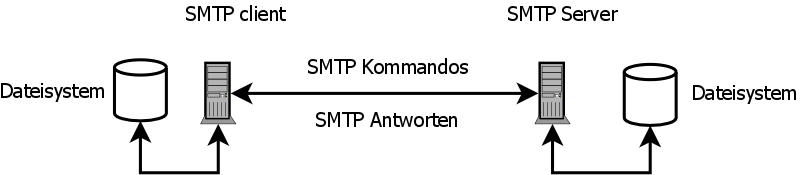
\includegraphics[scale=0.4]{Content/Intro/Protokolle/SMTP-Model.png}
	\caption{SMTP Modell}
	\label{fig:smtpmodel}
\end{figure}
